\chapter{GUI Reference}
\label{cha:ref}



%%%%%%%%%%%%%%%%%%%%%%%%%%%%%%%%%%%%%%%%%%%%%%%%%%%%%%%%%%%%%%%%%%%%%%%%%%%%%%%%%%%%%%%%%%%%%%%%%%%%%%%%%%%%%%%%%%%%%%%%%%%%%%%%%%%%%%%%%%%%%%%%%%%%%%%%%%
\section{Installation}
\label{sec:ref_install}

%%%%%%%%%%%%%%%%%%%%%%%%%%%%%%%%%%%%%%%%%%%%%%%%%%%%%%%%%%%%%%%%%%%%%%%%%%%%%
\subsection{Requirements}
\textbf{Hardware: }Ondex requires at least
\begin{itemize}
\item 2GHz CPU
\item 2GB RAM (4GB recommended)
\item 300 MB of free HDD space
\end{itemize}

\noindent\textbf{Operating system: }Ondex is a Java 6 application and therefore compatible with
\begin{itemize}
\item Windows XP / Vista / 7
\item Linux / UNIX / Solaris
\item Mac OS X 64-bit Intel (as this version supports Java 6)
\end{itemize}

\noindent\textbf{Software: }Ondex needs Java version 6 update 26 or later versions.
Make sure you have an adequate Java Runtime Environment installed on your system.
If not, you can download it from {\url{http://java.oracle.com}}.

Also make sure your PATH variable contains your java executable. 
To test whether this is the case, see section \ref{sec:testing_requirements} below.

%%%%%%%%%%%%%%%%%%%%%%%%%%%%%%%%%%%%%%%%%%%%%%%%%%%%%%%%%%%%%%%%%%%%%%%%%%%%%
\subsection{Installer}
There is an Ondex installer for Windows users. 
For Windows Vista / 7: Make sure NOT to install Ondex in ``C:$\backslash$Program Files (x86)''.

In the Ondex setup, the page ``Choose Components'' (see Figure \ref{fig:choose_components}) 
lets the user decide which features of Ondex they wish to install.
Several options are possible:
\begin{enumerate}
\item Ondex front-end plug-ins
\item Ondex front-end plug-ins (including experimental)
\item All Ondex front-end and Integrator plug-ins
\item All Ondex front-end and Integrator plug-ins (including experimental)
\item Custom
\end{enumerate}
The first option will allow users to use data visualisation tools which are stable.
The second option will allow users to use data visualisation tools which are stable as well as experimental.
The third option will allow users to use data visualisation and integration tools which are stable.
The fourth option will allow users to use data visualisation and integration tools which are stable as well as experimental.
The fifth option will allow users to customize their setup and manually select what they wish to install.
(For this fifth option, the plug-ins selected by default depend on what option out of the first four was last selected.)

\begin{figure}[H]
\centering
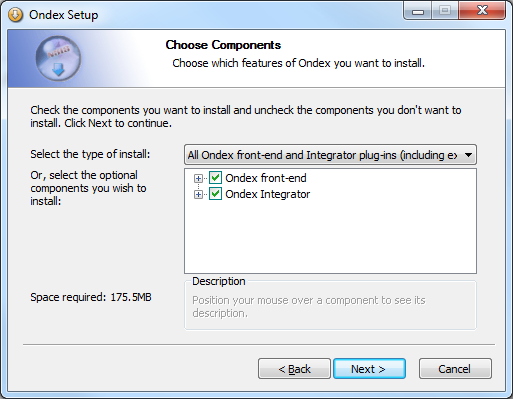
\includegraphics[scale=0.75]{images/Oct12/choose_components.png} 
\caption{Ondex Setup - Choose Components}
\label{fig:choose_components}
\end{figure}

During the installation, the Ondex setup (see figure \ref{fig:choose_memory}) 
will prompt the user to specify the default amount of memory Ondex should run with. 
This number should be set to 1200 for 32-bit systems with at least 2GB memory. 
For 64-bit systems it can be set to just under the amount of memory you have installed, 
\textit{e.g.} set it to 3500 on a system with 4GB of memory.

\begin{figure}[H]
\centering
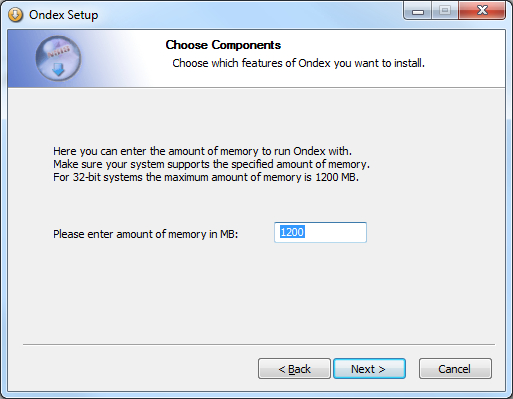
\includegraphics[scale=0.75]{images/Oct12/choose_memory.png} 
\caption{Ondex Setup - Configure memory}
\label{fig:choose_memory}
\end{figure} 

The installer will create shortcuts (which users can then access from the Start menu) unless stated otherwise during the setup.
Running the exe file for Ondex (using this shortcut or by double-clicking on it) will check that Java Runtime Environment version 1.6 or higher is installed.
If it is not, it will attempt to automatically download it.

Users of other operating systems may download the tar.gz file and execute the runme.sh file to start Ondex.
In Linux, a ``chmod 755 runme.sh'' might be needed to make the script executable from your user's account.



%%%%%%%%%%%%%%%%%%%%%%%%%%%%%%%%%%%%%%%%%%%%%%%%%%%%%%%%%%%%%%%%%%%%%%%%%%%%%
\subsection{Testing the requirements}
\label{sec:testing_requirements}

\textbf{WINDOWS: }
Click Start -$>$ Run enter ``cmd'' and press enter. 

\noindent\textbf{LINUX/GNOME: }
Right-click on your desktop and choose ``Open Terminal'' from the appearing context menu.

\noindent\textbf{LINUX/KDE: }
Choose ``Konsole'' from your Quick launcher.

Type ``java -version'' in the appearing console window and press enter.
If your system is configured correctly you will see a message that contains your current Java version. Make sure it is higher than version 1.6.
If you don't see a message, then you have either not installed Java yet, or you have not set your PATH variable.

%%%%%%%%%%%%%%%%%%%%%%%%%%%%%%%%%%%%%%%%%%%%%%%%%%%%%%%%%%%%%%%%%%%%%%%%%%%%%
\subsection{How to set the PATH variable}
\textbf{WINDOWS: }
Right-click on ``Computer'' in the start menu and choose ``Properties'' from the appearing context menu. 
Click on ``Advanced system settings'' on the left in the appearing window. 
Click the button ``Environment Variables'' on the bottom left of the window. 
You will see a list of variables with their assigned values. 
If the PATH variable already occurs in it, select it and click ``Edit''. 
Append a semicolon to the end of the value field and then enter the path to your Java binary directory. 
This is usually something like ``C:$\backslash$Program Files$\backslash$Java$\backslash$jdk1.6.0\_26$\backslash$bin''.
If the path contains any white spaces, make sure you put it in double quotes. 
If the variable PATH didn't exist yet on your system, create a new one and call it ``PATH''. 
Assign the binary path as it's value. However you don't need the semicolon in this case.

\noindent\textbf{LINUX: }
Go to your home directory and open the file ``.bashrc'' in your favourite editor. 
Append the line PATH=\$PATH:$<$javadir$>$ where $<$javadir$>$ is your path to the java binary directory, 
something like $/usr/java/latest/bin/$ to find out what it actually is you can execute the command ``type java'' in a console window. 

%%%%%%%%%%%%%%%%%%%%%%%%%%%%%%%%%%%%%%%%%%%%%%%%%%%%%%%%%%%%%%%%%%%%%%%%%%%%%
\subsection{To the attention of sysadmins}
A ``system-wide install'' of Ondex is discouraged because putting the Ondex directory tree 
in root space makes it hard for users to manage input, output, scripts and databases. 
Installing Ondex in users' spaces or creating an Ondex user is a good alternative. 

Databases will mostly have to be obtained by the sysadmin/users as flatfiles on a need-to-use basis. 
The expected location of those files is under $<$OndexDir$>$/data/importdata/ 
(where $<$OndexDir$>$ is the directory where Ondex was installed).

For a dataset which an average user is expecting to employ, it is essential to use a machine with enough memory.
It is also essential to increase the memory setting in the command line or runme file to run Ondex with more memory. 
Ondex's GUI can currently manage about 250,000 concepts and relations.
Limitations depend on available memory and CPU.

%%%%%%%%%%%%%%%%%%%%%%%%%%%%%%%%%%%%%%%%%%%%%%%%%%%%%%%%%%%%%%%%%%%%%%%%%%%%%
\subsection{Using Ondex behind a firewall}
In order to use Ondex when working behind a firewall, please modify the last line of runme.bat or runme.sh as follows:\\
\texttt{java -DproxySet=true -DproxyHost=your.proxy.com -DproxyPort=yourport -Dhttp.proxyUser=yourproxyuser -Dhttp.proxyPassword=yourproxypassword
-Xmx\%MEMORY\% -Dondex.dir=\%DATA\% -Dovtk.dir=\%OVTK\_DATA\% -Dplugin.scan.lib=false \ldots}

%%%%%%%%%%%%%%%%%%%%%%%%%%%%%%%%%%%%%%%%%%%%%%%%%%%%%%%%%%%%%%%%%%%%%%%%%%%%%%%%%%%%%%%%%%%%%%%%%%%%%%%%%%%%%%%%%%%%%%%%%%%%%%%%%%%%%%%%%%%%%%%%%%%%%%%%%%
\section{Loading Networks}
\label{sec:ref_loading}
It is possible to open biological networks in Ondex by:
\begin{itemize}
\item Importing network files.
\item Creating an empty network and manually adding concepts and relations.
\end{itemize}

\subsection{Loading Existing Biological Networks into Ondex}
Ondex can read files written in the following formats:
\begin{itemize}
\item oxl (Ondex XML, biological networks created using Ondex)
\item nwb (Network Workbench \url{http://nwb.cns.iu.edu/})
\item net (Pajek \url{http://pajek.imfm.si/doku.php?id=pajek})
\item cys (CytoScape \url{http://www.cytoscape.org})
\end{itemize}


\subsection{Creating an empty network and manually adding concepts and relations}
It is also possible to create a new, empty network and to manually add concepts and relations. 
To create an empty network, go to File -$>$ New. 
Click on the magic wand icon for ``Add a Concept or Relation'' or go to Edit -$>$ Concept / Relation -$>$ Add New.

If you wish to add a concept, click on ``Add a new Concept''. 
You will need to fill in all the fields highlighted in orange as they are compulsory. 
This will require creating Data Source and Concept Class identifiers and an Evidence Type.

If you wish to add a relation, click on ``Add a new Relation''. 
You will need to select concepts beforehand (shift + left mouse button to create a select area) 
so the drop-down lists offer these concepts as origin / target of the relation.
It maybe necessary to create a Relation Type identifier.

\subsection{Saving Files}
\label{sec:ref_sav}
You can save your Ondex files and export visualisations.
\begin{itemize}
\item To save a file, go to File -$>$ Save graph as. The panel on the right offers options
	\begin{itemize}
	\item Save invisible concepts/relations: if hidden items have not been deleted from the graph yet, you can untick this option to delete them before saving.
	\item Save appearance: will save colours, shapes, sizes and layout of concepts and relations.
	\end{itemize}
\item To save images from the visualization window, go to File -$>$ Save image as
	\begin{itemize}
	\item Select an export format from the list
	\item Scale factor: will scale the visualisation by the given factor before saving
	\end{itemize}
\item To export the graph to another format, go to File -$>$ Export
	\begin{itemize}
	\item Select an export format from the list
	\item Scale factor (only applicable to some export formats)
	\end{itemize}
\end{itemize}

%%%%%%%%%%%%%%%%%%%%%%%%%%%%%%%%%%%%%%%%%%%%%%%%%%%%%%%%%%%%%%%%%%%%%%%%%%%%%%%%%%%%%%%%%%%%%%%%%%%%%%%%%%%%%%%%%%%%%%%%%%%%%%%%%%%%%%%%%%%%%%%%%%%%%%%%%%
\section{Metagraph}
\label{sec:ref_metagraph}

The Metagraph view has 2 buttons at the bottom of its window:
\begin{itemize}
\item Legend: will pop up a window which displays a modifiable colour/shape legend as well as 
the number of concepts and relations in the network for concept classes, data sources, relation types and evidence types
\item Main Network: will open the main network visualisation window if it was minimized 
\end{itemize}

The Metagraph view has its own menu system:
\begin{itemize}
\item File
	\begin{itemize}
	\item Export: will export the metagraph as an image (see Section \ref{sec:ref_sav} for more information)
	\end{itemize}
\item Edit
	\begin{itemize}
	\item Show All/Selection: Set items on the metagraph to visible - All or a selection (select using left click, press shift to select several items)
	\item Hide All/Selection: Set items on the metagraph to invisible - All or a selection (select using left click, press shift to select several items)
	\end{itemize}
\item Appearance
	\begin{itemize}
	\item Labels: show the labels of meta concepts / meta relations on the metagraph
	\item Config: change the meta relation thickness, meta concept size and font size showing on the metagraph
	\item Scale to Fit: after resizing the window, will scale the metagraph to fit it
	\item Refresh Layout: will draw the metagraph again should users have moved anything and will end with a ``Scale to Fit''
	\item Load Appearance: loads previously saved layout and sizes of the metagraph
	\item Save Appearance: saves current layout and sizes of the metagraph  
	\end{itemize}
\end{itemize}

%%%%%%%%%%%%%%%%%%%%%%%%%%%%%%%%%%%%%%%%%%%%%%%%%%%%%%%%%%%%%%%%%%%%%%%%%%%%%%%%%%%%%%%%%%%%%%%%%%%%%%%%%%%%%%%%%%%%%%%%%%%%%%%%%%%%%%%%%%%%%%%%%%%%%%%%%%
\section{Manipulating Networks}
\label{sec:ref_manipulating}

There are several ways of manipulating networks in Ondex:

\begin{itemize}

\item Zooming
Ondex provides two mechanisms for zooming:
\begin{itemize}
\item Using the mouse - move the mouse scroll forwards and backwards (the graph moves towards you and away from you respectively)
\item Using the two zoom buttons on the toolbar to zoom in and out of the network (or Appearance -$>$ Zoom)
\item Using a combination of the mouse and the zoom buttons, you can zoom in on a group of concepts -
press shift to select a few concepts with the left mouse button, zoom in on the selected group
\end{itemize}

\item Selecting an area to look at from the overview
When studying large graphs, using the View -$>$ Satellite View to move and navigate across the network can be very useful.

\item Manually rearrange a network
Select the concepts of interest and move them around. See last exercise (and help points) in Section \ref{sec:loading}.

\item Automatically rearrange a network
There are a variety of layout algorithms which can be found in the Appearance -$>$ Layouts menu. 
The Gem layout is the most popular one.

\item Rotating and Sheering your network
Finally you can rotate and scale your network within Ondex. 
In the transforming mode (See Section \ref{sec:ref_icons} for icon or, in the menus, Edit -$>$ Mouse Mode), 
shift + mouse will rotate and control + mouse will sheer your graph.
\end{itemize}


%%%%%%%%%%%%%%%%%%%%%%%%%%%%%%%%%%%%%%%%%%%%%%%%%%%%%%%%%%%%%%%%%%%%%%%%%%%%%%%%%%%%%%%%%%%%%%%%%%%%%%%%%%%%%%%%%%%%%%%%%%%%%%%%%%%%%%%%%%%%%%%%%%%%%%%%%%
\section{Buttons in toolbar}
\label{sec:ref_icons}

The toolbar is composed of several icons followed by a search bar which is explained in further details in Section \ref{sec:search}.
It is possible to undock this toolbar by a simple ``drag and drop''. 
When it is undocked, it is possible to re-dock it by clicking on its far left side and again dragging and dropping to its original position.

\begin{figure}[H]
\centering

\includegraphics[scale=0.7]{images/Oct12/icon_bar.png} 
\caption{Ondex icon bar}
\label{fig:icon_bar}
\end{figure}

\begin{figure}[H]
\centering

\includegraphics[scale=0.9]{images/Oct12/icon_open_save.png} 
\caption{The ``open'' icon on the left and the ``save'' icon on the right. Also available from the File menu.}
\label{fig:icon_open_save}
\end{figure}

\begin{figure}[H]
\centering

\includegraphics[scale=0.9]{images/Oct12/icon_add_i_v.png} 
\caption{The ``Add a Concept or Relation'' on the left, the ``Information on selected Concept or Relation'' icon in the middle 
and the ``Edit selected Concept or Relation'' on the right.
Available in the menus from Edit -$>$ Concept / Relation -$>$ Add New, View -$>$ Item Info, Edit -$>$ Concept / Relation -$>$ Edit Selected.}
\label{fig:icon_add_i_v}
\end{figure}

\begin{figure}[H]
\centering

\includegraphics[scale=0.9]{images/Oct12/icon_del_clone.png} 
\caption{The ``Delete selected Concept or Relation'' icon on the left and the ``Copy whole Network as new'' icon on the right.
Available in the menus from Edit -$>$ Concept / Relation -$>$ Delete Selected and Edit -$>$ Clone Network.}
\label{fig:icon_del_clone}
\end{figure}

\begin{figure}[H]
\centering

\includegraphics[scale=0.9]{images/Oct12/icon_refresh_zoom2_center.png} 
\caption{The ``Refresh Layout'', ``Zoom In'', ``Zoom Out'' and ``Center Network'' icons from left to right.
Available in the menus from Appearance -$>$ Refresh Layout, Appearance -$>$ Zoom, Appearance -$>$ Center Network.}
\label{fig:icon_refresh_zoom2_center}
\end{figure}

\begin{figure}[H]
\centering
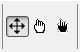
\includegraphics[scale=0.9]{images/Oct12/icon_mouse_modes.png} 
\caption{The left-hand side icon sets the mouse to ``transforming'' mode (to move within the network) whereas the
white hand icon sets the mouse to ``picking'' mode (to select concepts, drag and drop them).
When a graph is not dense, the two modes interchange depending on the position of the mouse (positioned over blank or over concept or relation).
When a graph is dense, manually selecting a mode can be useful.
The black hand sets the mouse to ``annotating'' mode for annotation purposes.
All available from Edit -$>$ Mouse mode.}
\label{fig:icon_mouse_modes}
\end{figure}


%%%%%%%%%%%%%%%%%%%%%%%%%%%%%%%%%%%%%%%%%%%%%%%%%%%%%%%%%%%%%%%%%%%%%%%%%%%%%%%%%%%%%%%%%%%%%%%%%%%%%%%%%%%%%%%%%%%%%%%%%%%%%%%%%%%%%%%%%%%%%%%%%%%%%%%%%%
\section{Search bar in toolbar}
\label{sec:ref_search}
Ondex includes a Search feature, which enables you to quickly find concepts by searching their names, accessions and other properties. 
The default mode of the Search feature is Keyword search, other modes like chemical similarity or UniProt identifier are also available.

\begin{figure}[H]
\centering
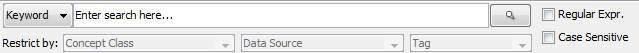
\includegraphics[scale=0.7]{images/Oct12/search_bar.png} 
\label{fig:search_bar}
\caption{Search bar}
\end{figure}

If you select (single click) one item in the search results, you will need to click on the icon ``Zoom In'' in order for Ondex to zoom in on this particular concept. 
You can then use the mouse scroll functionality to get to the concept.
If you select several items (using the Control key) in the search results, Ondex will automatically zoom in to show all those items as close up as possible.

\textbf{Configuring an Ondex Search }
\begin{itemize}
\item At the end of the toolbar in Keyword search mode, there are 2 options that can be configured for each search. 
If you tick ``Regular Expr.'', you may enter a JAVA regular expression. An example would be: p$\backslash$$\backslash$d\{1,4\}.
It will match a ``p'' followed by 1 to 4 digits. 
For more information on regular expressions in JAVA, please visit \url{http://docs.oracle.com/javase/tutorial/essential/regex/}.
If you tick ``Case Sensitive'', the search will be sensitive to lower/upper case of each character.
\item Under the search box, there are 3 drop-down lists which allow users to restrict their search (by Concept Class, Data Source or Tag).
\end{itemize}


%%%%%%%%%%%%%%%%%%%%%%%%%%%%%%%%%%%%%%%%%%%%%%%%%%%%%%%%%%%%%%%%%%%%%%%%%%%%%%%%%%%%%%%%%%%%%%%%%%%%%%%%%%%%%%%%%%%%%%%%%%%%%%%%%%%%%%%%%%%%%%%%%%%%%%%%%%
\section{Menu system}
\label{sec:ref_menus}
 
\subsection{File}
\label{sec:menu_file}
The File menu contains basic file functionality.
\begin{itemize}
\item New: creates a new empty network 
\item Open: opens an Ondex network from a file
\item Import Expression Data: launches a wizard to import data from a tab, space or comma delimited file into the network 
\item Save graph as: saves Ondex network in a file
\item Save image as: saves the visualisation content as an image
\item Import: imports files in certain network formats, see \ref{sec:ref_loading}
\item Export: exports network to certain formats, see \ref{sec:ref_sav}
\item Print: prints the visualisation window content
\item Exit: exits Ondex
\end{itemize}

\subsection{Edit}
\label{sec:menu_edit}
\begin{itemize}
\item Undo: to undo last change (only available on right-click actions and filters)
\item Undo All: to undo all changes (same restriction)
\item Redo: to redo last change (only available on right-click actions and filters)
\item Redo All: to redo all changes (same restriction)
\item Revert Visibility to Last Save: to go back to the way the graph was the last time it was saved
\item Labels: to change concept label font, composition (to allow for various names to be displayed next to each concept on the graph) or to change relation label font
\item Delete Hidden Items: to remove invisible items from the network
\item Concept / Relation -$>$ Add New, Edit Selected, Delete Selected
\item Mouse Mode -$>$ Transforming, Picking, Annotating (see end of Section \ref{sec:ref_icons})
\item Clone Network: to copy whole network as new (useful to do comparisons)
\item Settings: to set up notifications or auto-save of graph (as well as login information for developers only)
\end{itemize}

\subsection{View}
\label{sec:menu_view}
\begin{itemize}
\item Metagraph: to display a metagraph containing all the types of concepts/relations contained in the main network
\item Legend: to modify colours/shapes of concepts/relations
\item Item Info: to display information on selected items (concepts/relations) of the network
\item List: to display a list of all concepts or relations (also allows users to choose which labels to display)
\item Tabular Graph Editor: to edit concepts and relations using tables (rather than the graph)
\item Satellite View: to open a movable overview of the network
\item Windows: to view a list of all the windows opened in Ondex (also allows users to display, minimize, maximize or close all windows)
\end{itemize}


\subsection{Appearance} 
\label{sec:menu_app}
\begin{itemize}
\item Labels: to shows the names of concepts/relations/both on the main network
\item Layouts: a collection of algorithms to organise networks visually (described below)
\item Colour Concepts:
 \begin{itemize}
 \item by Data Source:
 colours concepts based on their data source
 \item by Concept Class:
 colours concepts based on their concept class
 \item by Evidence Type:
 colours concepts based on their evidence type
 \end{itemize}
\item Colour Relations:
 \begin{itemize}
 \item by Relation Type:
 colours relations based on their relation type
 \item by Evidence Type:
 colours relations based on their evidence type
 \end{itemize}
\item Shape Relations:
\begin{itemize}
 \item using Quad Curves
 \item using Cubic Curves
 \item using Bent Lines
 \item using Straight Lines
 \item Draw arrows (untick to remove arrows on relations)
 \end{itemize}
\item Smooth Relations: anti-aliasing painting of relations in the network
\item Show MouseOver: enable mouse over display of chemical drawings on nodes
\item Update Display: to update the visualisation window with recent modifications
\item Load Appearance: to load some or all items of appearance that had been previously saved
\item Save Appearance: to save layout, concept colours, concept shapes, concept sizes, relation colours and relation widths
\item Center Network: centers the network within the visualisation window
\item Refresh Layout: to get back to the latest layout that was drawn (e.g. useful after moving concepts and relations around)
\item Zoom: zoom in or out
\end{itemize}


\subsubsection{Layouts:}
\begin{itemize}
\item Circular:
for a circular arrangement corresponding to concept classes
\item Gem:
for the Gem layout algorithm\footnote{
Frick A., Ludwig A. and Mehldau H. (1994). ``A Fast Adaptive Layout Algorithm for Undirected Graphs (Extended Abstract and System Demonstration)''. 
Lecture Notes In Computer Science; Vol. 894. Proceedings of the DIMACS International Workshop on Graph Drawing, 388--403.}:
\item More:
  \begin{itemize}
  \item Connectivity:
  for a mixture of the circular and hierarchical layouts
  \item Flip:
  for a flip around of selected concepts (mirror effect)
  \item Force Directed:
  for a force-directed algorithm based on attributes values
  \item Genomics:
  for a view of the data where chromosomes are represented as batons
  \item Hierarchical:
  for a hierarchy arranged by concept classes
  \item Kamada-Kawai:
  for the Kamada-Kawai layout algorithm\footnote{Kamada T. and Kawai S. (1989). ``An algorithm for drawing general undirected graphs.'' Information Processing Letters, 31, 7--15.}
  \item LinLog:
  for the LinLog layout algorithm\footnote{\url{http://www.informatik.tu-cottbus.de/~an/GD/linlog.html}}
  \item Radial Tree:
  for a layout determined by tree extraction and polar coordinates
  \item Relation Type Specific:
  for a force-directed algorithm based on relation types
  \item Static:
  for the latest saved layout
  \item Sugiyama:
  for the Sugiyama layout algorithm\footnote{Sugiyama, K. and Misue, K. ``Visualization of structural information: Automatic drawing of compound digraphs'', 1991.}
  \item Tree:
  for a directed rooted tree
  \end{itemize}
\item Layout Options:
for options on the parameters of some algorithms (some algorithms do not have options, others do but are not yet supported)
\end{itemize}


\subsection{Tools}
\label{sec:menu_tools}
\begin{itemize}
\item Integrator: user interface to allow users to create their own data integration pipeline (see Section \ref{sec:integrator})
\item Filters: a collection of algorithms to make some concepts/relations invisible (described below)
\item Annotators: a collection of algorithms to visualise the data held on concepts/relations (described below)
\item Selecting Concepts/Relations: this submenu allows users to select all concepts/relations on the network, or invert their original selection
\item Console: a scripting console (see Section \ref{sec:parsing_tabdel}) 
\item Popup Editor: create JavaScript based custom right click functionality 
\item Statistics: displays statistics about the opened network
\end{itemize}


\subsubsection{Filters:}
   \begin{itemize}
   \item Neighbourhood: to see a particular number of neighbours only around a particular concept 
   \item Tag: narrows down the graph to all concepts which were annotated with the same tag
   \item Unconnected: filters out all unconnected concepts
   \item More:
	\begin{itemize}
	\item Attribute Value Matcher: filters out concepts or relations based on a given attribute and value
	\item Concept Class: filters out some particular class of concepts
	\item Data Source: filters out concepts from a specified data source
	\item Defluff: filters out single-linked chains that otherwise end in unconnected concepts
	\item Degree: filters out concepts that have a number of ingoing/outgoing relations that is less than, equal or greater than the numbers set by the user in the filter window
	\item Evidence Type: filters out concepts from a specified evidence type
	\item Genomics: shows only genes of the specified regions and their neighbourhood
	\item Missing Relation Type: filters out concepts which are missing a specified type of relation
	\item Relation Type: filters out some particular type of relations
	\item Scatter Plot: filters concepts according to two attributes values selected in a scatter plot 
	\item Shortest Paths:
	  \begin{enumerate}
	  \item All Pairs Shortest Path:
	  computes the shortest paths between all possible pairs of concepts and removes all relations that are not part of these shortest paths
	  \item Shortest Path:
	  computes the Dijkstra shortest path algorithm from a particular concept 
	  \item Single Shortest Path:
	  computes the shortest path between two given concepts
	  \end{enumerate}
	\item SubGraph:
	filters out all concept classes and relation types that are not selected by the user in this sort of metagraph (from a concept selected by the user to start with)
	\item Threshold:
	selects a threshold for one of the concepts attributes' value
	\end{itemize}
   \end{itemize}

\subsubsection{Annotators:}
   \begin{itemize}
   \item Colour Concepts by General Attribute: to colour concepts based on one of their attribute's value
   \item Scale Concepts by Numerical Value: to resize concepts based on one of their attribute's value
   \item Scale/Colour Concepts by Numerial Value: to resize and colour concepts based on one of their attribute's numerical value
   \item Scale/Colour Relations by Numerial Value: to resize and colour relations based on one of their attribute's numerical value
   \item Shape Concepts by General Attribute: to shape concepts based on one of their attribute's value
   \item More:
      \begin{itemize}
      \item Betweenness / Degree Centrality:
      to resize concepts based on their degree centrality (or hub-likeness) and change their colour depending on their betweenness centrality 
      (or how influential they are) within the network
      \item Betweenness Centrality:
      to resize concepts based on how influential they are within the network\footnote{
      Brandes U. (2001). ``A faster algorithm for betweenness centrality.'' Journal of Mathematical Sociology, Vol. 25, 163-177.}
      \item Chemical Drawings:
      to display chemical drawings on nodes which hold chemical data structure
      \item Cluster Complexity:
      Identifies all maximal cliques in a graph and ranks them according to their Shannon entropy (in physics: "disorder" of a system) measure for a given attribute 
      (for example different phenotypes in a clique). Displays the ranking and allows for selection of interesting cliques.
      \item Colour Concepts with Series Data:
      Colours concepts according to a list of numerical attributes. 
      The user can iterate over this list to select the attribute mapped to concept colour. 
      For example, iterating through expression values of different time points of a micro-array experiment one after the other.
      \item Colour Relations by Concept Tag Intersection:
      to colour relations green if the two concepts they link have more than one tag in common, red otherwise
      \item Concept Degree:
      Creates attributes ("IN\_DEGREE", "OUT\_DEGREE", "BOTH\_DEGREE") on the concepts which reflect the in- and out-degrees of the node corresponding to the concept. 
      This annotator does not change the visualisation of the graph (please apply the Attribute Value Matcher filter to do so).
      \item Degree Specificity:
      Creates attributes on the concepts and/or relations which reflect a certain set of concept class connectivity.
      \item Display Series Data on Concepts:
      Draw line or bar graphs on the nodes in the network, visualising the time series data selected.
      \item Graph Algorithms:
      to select one of five algorithms (all cliques, connected components, cut
      concepts, minimum equivalent, strongly connected). 
      Results are added as attributes to the concepts.
      \item Relation Betweenness Clusterer:
      Adds an attribute (true/false) to a chosen number of relations that have the highest betweenness measure. 
      This annotator does not change the visualisation of the graph (please apply a filter to do so). 
      After applying a filter (e.g. the Attribute Value Matcher filter), the graph would show highly connected components.
      \item Scale Concepts/Relations by Type:
      to choose the size of concepts/relations for each concept class and relation type
      \item Virtual Knock-Out:
      to remove one concept at a time virtually and calculating the structure changes in the network
      \item Weighting Relation Attribute:
      to add an attribute to relations which corresponds to a weighted calculation of the existing attributes (only works on networks where all relations have attributes)
      \end{itemize}
   \end{itemize}

\subsection{Help}
\label{sec:menu_help}
\begin{itemize}
\item About: a brief message about the project
\item Documentation: a documentation of Ondex functions with screenshots
\item Report a problem: Error reporting dialog to submit additional information
\item Tutorial: this tutorial is available in PDF format through this menu
\item Version: Current program version and system information
\item Welcome message: the welcome message which shows when starting Ondex
\end{itemize}



%%%%%%%%%%%%%%%%%%%%%%%%%%%%%%%%%%%%%%%%%%%%%%%%%%%%%%%%%%%%%%%%%%%%%%%%%%%%%%%%%%%%%%%%%%%%%%%%%%%%%%%%%%%%%%%%%%%%%%%%%%%%%%%%%%%%%%%%%%%%%%%%%%%%%%%%%%
\newpage
\section{Integrator}
\label{sec:ref_integrator}
The Ondex Integrator is Ondex's workflow manager. It is available from the Tools menu and looks like this
\begin{figure}[H]
\centering
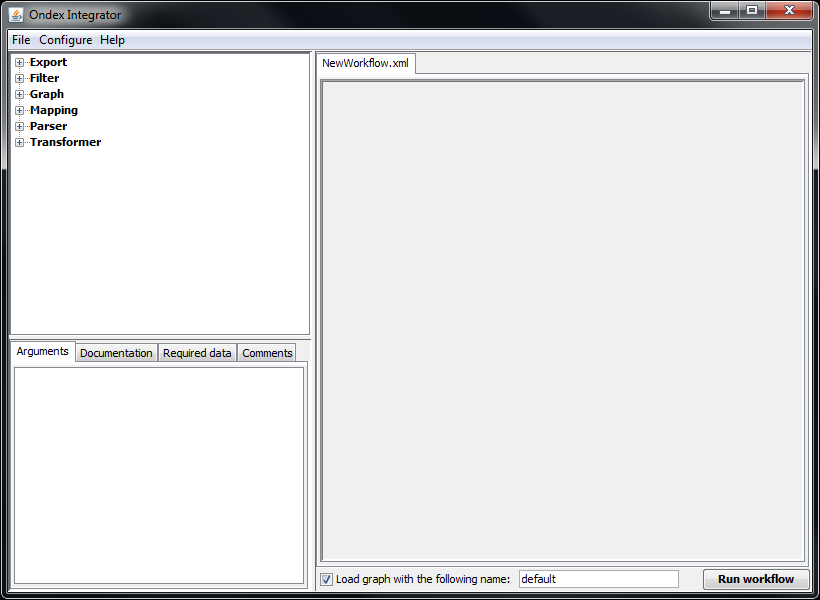
\includegraphics[scale=0.55]{images/Oct12/integrator.png} 
\caption{Integrator}
\label{fig:integrator}
\end{figure}
There 3 main areas to the Ondex Integrator (which are all adjustable using the mouse):
\begin{itemize}
\item Top left: listing panel.
This window lists all the plugins available to add to your workflow.
\item Bottom left: documentation panel.
This window contains 4 tabs and shows documentation for the selected item (single click) in the listing panel above.
\item Right: workflow panel.
Selected plugins (double click) will appear in this window for you to set parameters.
\end{itemize}

Other useful points:
\begin{itemize}
\item File -$>$ Validate allows users to check their workflow before running it.
\item Configure -$>$ ``Show stable plugins only'' can be ticked/unticked to hide/show experimental plugins as well.
\item There is a ``Run workflow'' button at the bottom-right corner. Saving your workflow before running is advised (File -$>$ Save As).
Running the workflow will highlight the name of the plugins in yellow (while running), green (when finished).
A error report pops up when error(s) are found. A ``$>>$'' icon is placed next to each error to show users where each of them is in the pipeline.
The name of the workflow becomes
\begin{itemize}
\item orange while it is running
\item red if running has failed 
\item back to black if it completed successfully
\end{itemize}
\end{itemize}

%Information on the plugins themselves can be found on \url{http://ondex.rothamsted.ac.uk/ondex-plugins/list}.


%%%%%%%%%%%%%%%%%%%%%%%%%%%%%%%%%%%%%%%%%%%%%%%%%%%%%%%%%%%%%%%%%%%%%%%%%%%%%%%%%%%%%%%%%%%%%%%%%%%%%%%%%%%%%%%%%%%%%%%%%%%%%%%%%%%%%%%%%%%%%%%%%%%%%%%%%%
\section{Console}
\label{sec:ref_console}
The console is Ondex's scripting interface. It is available from the Tools menu and looks like this
\begin{figure}[H]
\centering
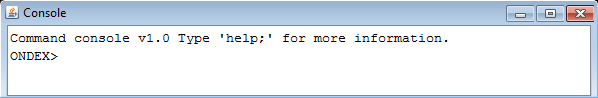
\includegraphics[scale=0.7]{images/Oct12/console.png} 
\caption{Console}
\label{fig:console}
\end{figure}
Section \ref{sec:parsing_tabdel} explains how to import tab-delimited data files using it.

%%%%%%%%%%%%%%%%%%%%%%%%%%%%%%%%%%%%%%%%%%%%%%%%%%%%%%%%%%%%%%%%%%%%%%%%%%%%%%%%%%%%%%%%%%%%%%%%%%%%%%%%%%%%%%%%%%%%%%%%%%%%%%%%%%%%%%%%%%%%%%%%%%%%%%%%%%
\section{Statistics}
\label{sec:ref_stats}
The statistics module is available from the Tools menu.
You see a window that is divided into 3 main areas as shown in Figure \ref{fig:stats}.
\begin{itemize}
\item Top left: listing panel.
It contains 4 lists with different graph elements that can be used as variables or filters.
\item Top right: selection panel.
It contains the variable field (with two buttons that load it with the currently selected element or unload it, respectively).
The filters list is below the variable field (same buttons to load/unload).
Select from the listing panel and enter in value(s) of your choice.
They will be handled as conditions linked with an ``or'' operation.
\item Bottom: display panel.
It shows the number of concepts that were found that meet the selected conditions and the respective number of relations.
In case the variable is a numerical value, it also features the mean and the standard deviation values, and a histogram.
\end{itemize}

\begin{figure}[H]
\centering
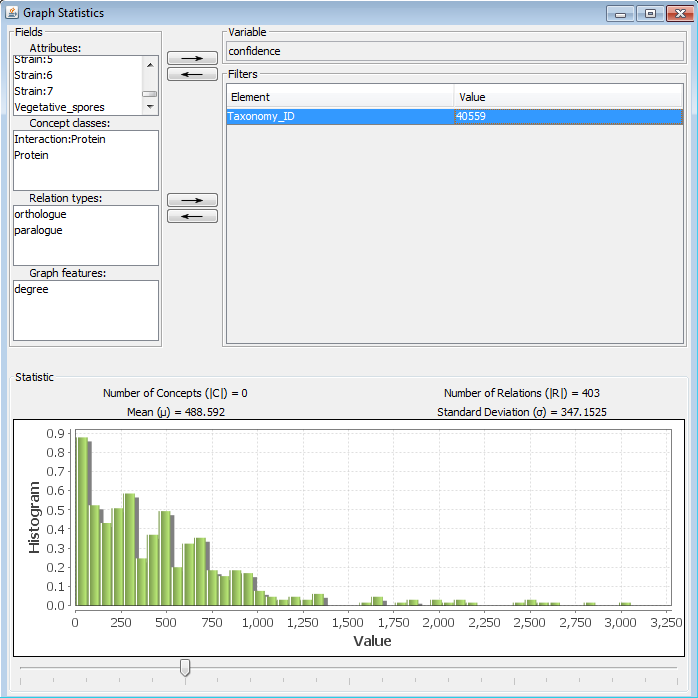
\includegraphics[scale=0.6]{images/Oct12/stats.png} 
\caption{Statitics module}
\label{fig:stats}
\end{figure}

